\documentclass[12pt]{article}

\usepackage{amsmath}
\usepackage{amssymb}
\usepackage{calc}
\usepackage{units}
\usepackage{graphicx}
\usepackage[pdftex]{hyperref}
\usepackage{subfig}
\usepackage[margin=1in]{geometry}
\usepackage{listings}
\usepackage[numbers,sort&compress]{natbib}
\usepackage{bm}
\usepackage{paralist}
\usepackage[draft]{fixme}
\usepackage{textcomp}

\hypersetup{
  breaklinks=true,
  pdftitle={The Electrical Properties of Materials: Resistivity},
  pdfauthor={Kevin R. Lynch based on a lab by E.M.Levin}, 
  pdfsubject={Phyiscs, Electricity and magnetism},
  pdfkeywords={resistance, resistivity, tungsten, copper},
  pdflang={en-US},
}

\title{The Electrical Properties of Materials: Resistivity}
\author{}
%Kevin R. Lynch, based on an earlier lab by E.M.Levin
%\date{2012-02-3}
\date{}

\begin{document}

\maketitle

\section{Objectives}
\label{sec:objectives}

\begin{enumerate}
\item To understand the properties of resistance and resistivity in
  conductors, 
\item To measure the resistivity and temperature coefficient of
  tungsten, and
\item To design and implement a resistivity measurement experiment. 
\end{enumerate}

\section{Introduction}
\label{sec:introduction}

In previous lab(s) you have measured the resistance of different
objects via different methods.  You have also used the known
resistances of objects to make predictions about voltages across and
currents through those objects.  After a few moments thought, however,
it should be clear that the resistance of an object is not a
fundamental property of the materials the object is constructed from:
it is a derived property that depends not only on the
\textit{material}, but also on the \textit{geometry} of the material.
The analogy of current flow to fluid flow is apt here: recall from our
study of fluid dynamics last semester that water has an ``easier''
time flowing through a short or large diameter pipes than through long
or small diameter pipes.

The resistance of an object, then, is not a fundamental property of
the material: it is derived, or extrinsic.  From studying how
resistance varies with shape (geometry), you can determine that there
is a property of the material that is fundamental, or intrinsic, to
the material.  We call this property
\textit{resistivity}.\footnote{The inverse of resistivity is also
  given a name, the \textit{conductivity}.  In some older physics
  texts and in more engineering oriented texts, you may see these
  referred to as ``specific resistance'' and ``specific conductance'',
  in analogy with the thermodynamic properties of ``heat capacity''
  and ``specific heat''.}

While we consider resistivity an intrinsic property of the material,
that does not mean it is a constant!  Under different temperature
conditions, for instance, the resistivity changes.  In this lab, you
will explore the properties of resistivity of various materials.

\section{Theory}
\label{sec:theory}

The resistance of a real (as opposed to an ideal) conductor of uniform
cross section is given in terms of the resistivity, $\rho$, length,
$L$, and cross-sectional area, $A$, by the relation
\begin{gather}
  R = \rho \frac{L}{A}\ .
\label{eq:resistivity}
\end{gather}
This is a \textit{single} relation between \textit{four} variables; if
you know any three of them, you can calculate the fourth.  Dimensional
analysis should convince you that the SI units of resistivity are
$\unit{\Omega \cdot m}$.

The resistivity of a material depends on the temperature.  In general,
much as the length of a material increases with temperature, so does
the resistivity.  Detailed models of the temperature dependence of
resistivity are very complicated.  However, if you look over a narrow
temperature range, you can model the temperature dependence with a
linear function, just as you did for the temperature dependence of
length. So, if $\rho_1$ and $\rho_2$ are the resistivities at
temperatures $T_1$ and $T_2$ respectively, you can say
\begin{gather*}
  \rho_2 = \rho_1 \left(1 + \alpha (T_2 - T_1) \right)\ ,
\end{gather*}
where $\alpha$ is an empirically (experimentally) determined
parameter called the \textit{temperature coefficient of resistivity}.

\section{Procedures}
\label{sec:procedures}

This lab has two parts: a scripted study of the resistivity of
tungsten (Section~\ref{sec:incandescent}, and a more free-form
determination of the resistivity of various materials.  In the latter
section, we do not give you detailed instructions: you are responsible
for both designing the experiment, and 

\subsection{The Incandescent Bulb}
\label{sec:incandescent}

\begin{figure}
  \centering
  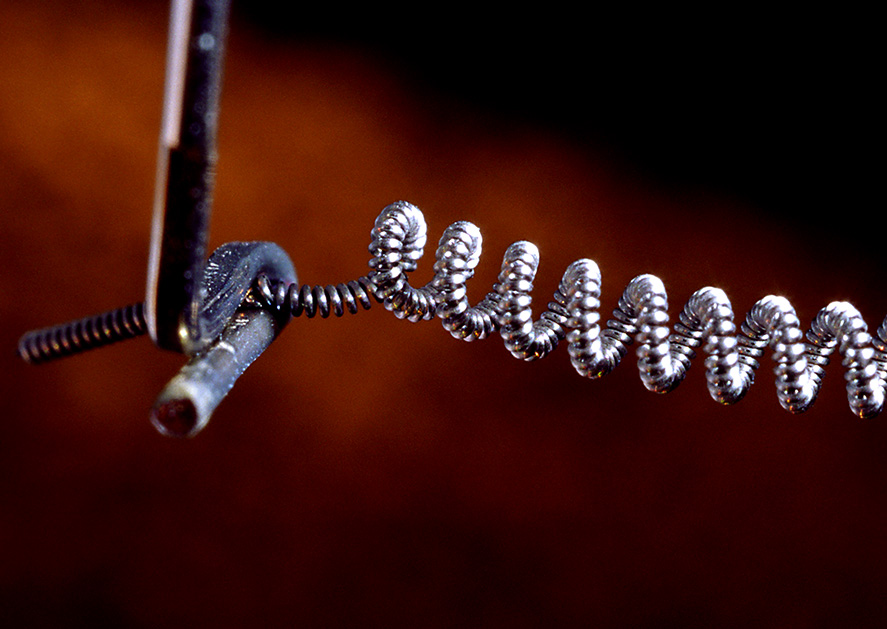
\includegraphics[width=2\textwidth/3]{figures/filament}
%% Figure in public domain:
%% http://en.wikipedia.org/wiki/File:Filament.jpg
  \caption{The coiled coil of an incandescent bulb filament.}
  \label{fig:filament}
\end{figure}
An incandescent bulb consists of a coiled coil of tungsten wire, which
has a very small coefficient of thermal expansion.  When you apply an
electrical current, the filament - which is just a resistor, after all
- dissipates power according to the relation
\begin{gather}
  P = VI\ ,
\label{eq:power}
\end{gather}
and heats to a few thousand degrees Celsius.  As you recall from
Physics I, hot objects emit electromagnetic radiation; the tungsten
filaments are designed to emit as large a fraction of their power in
the optical spectrum as possible - i.e. as visible light.

Light bulbs are labeled for sale according not to the amount of light
they emit, or their resistance, but to their power dissipation (``We
need to buy more \unit[60]{W} light bulbs.'').  This rating assumes
that the bulb will be operated at a fixed \unit[120]{V}; what happens
to the power dissipation at other operating voltages?

\begin{figure}
  \centering
  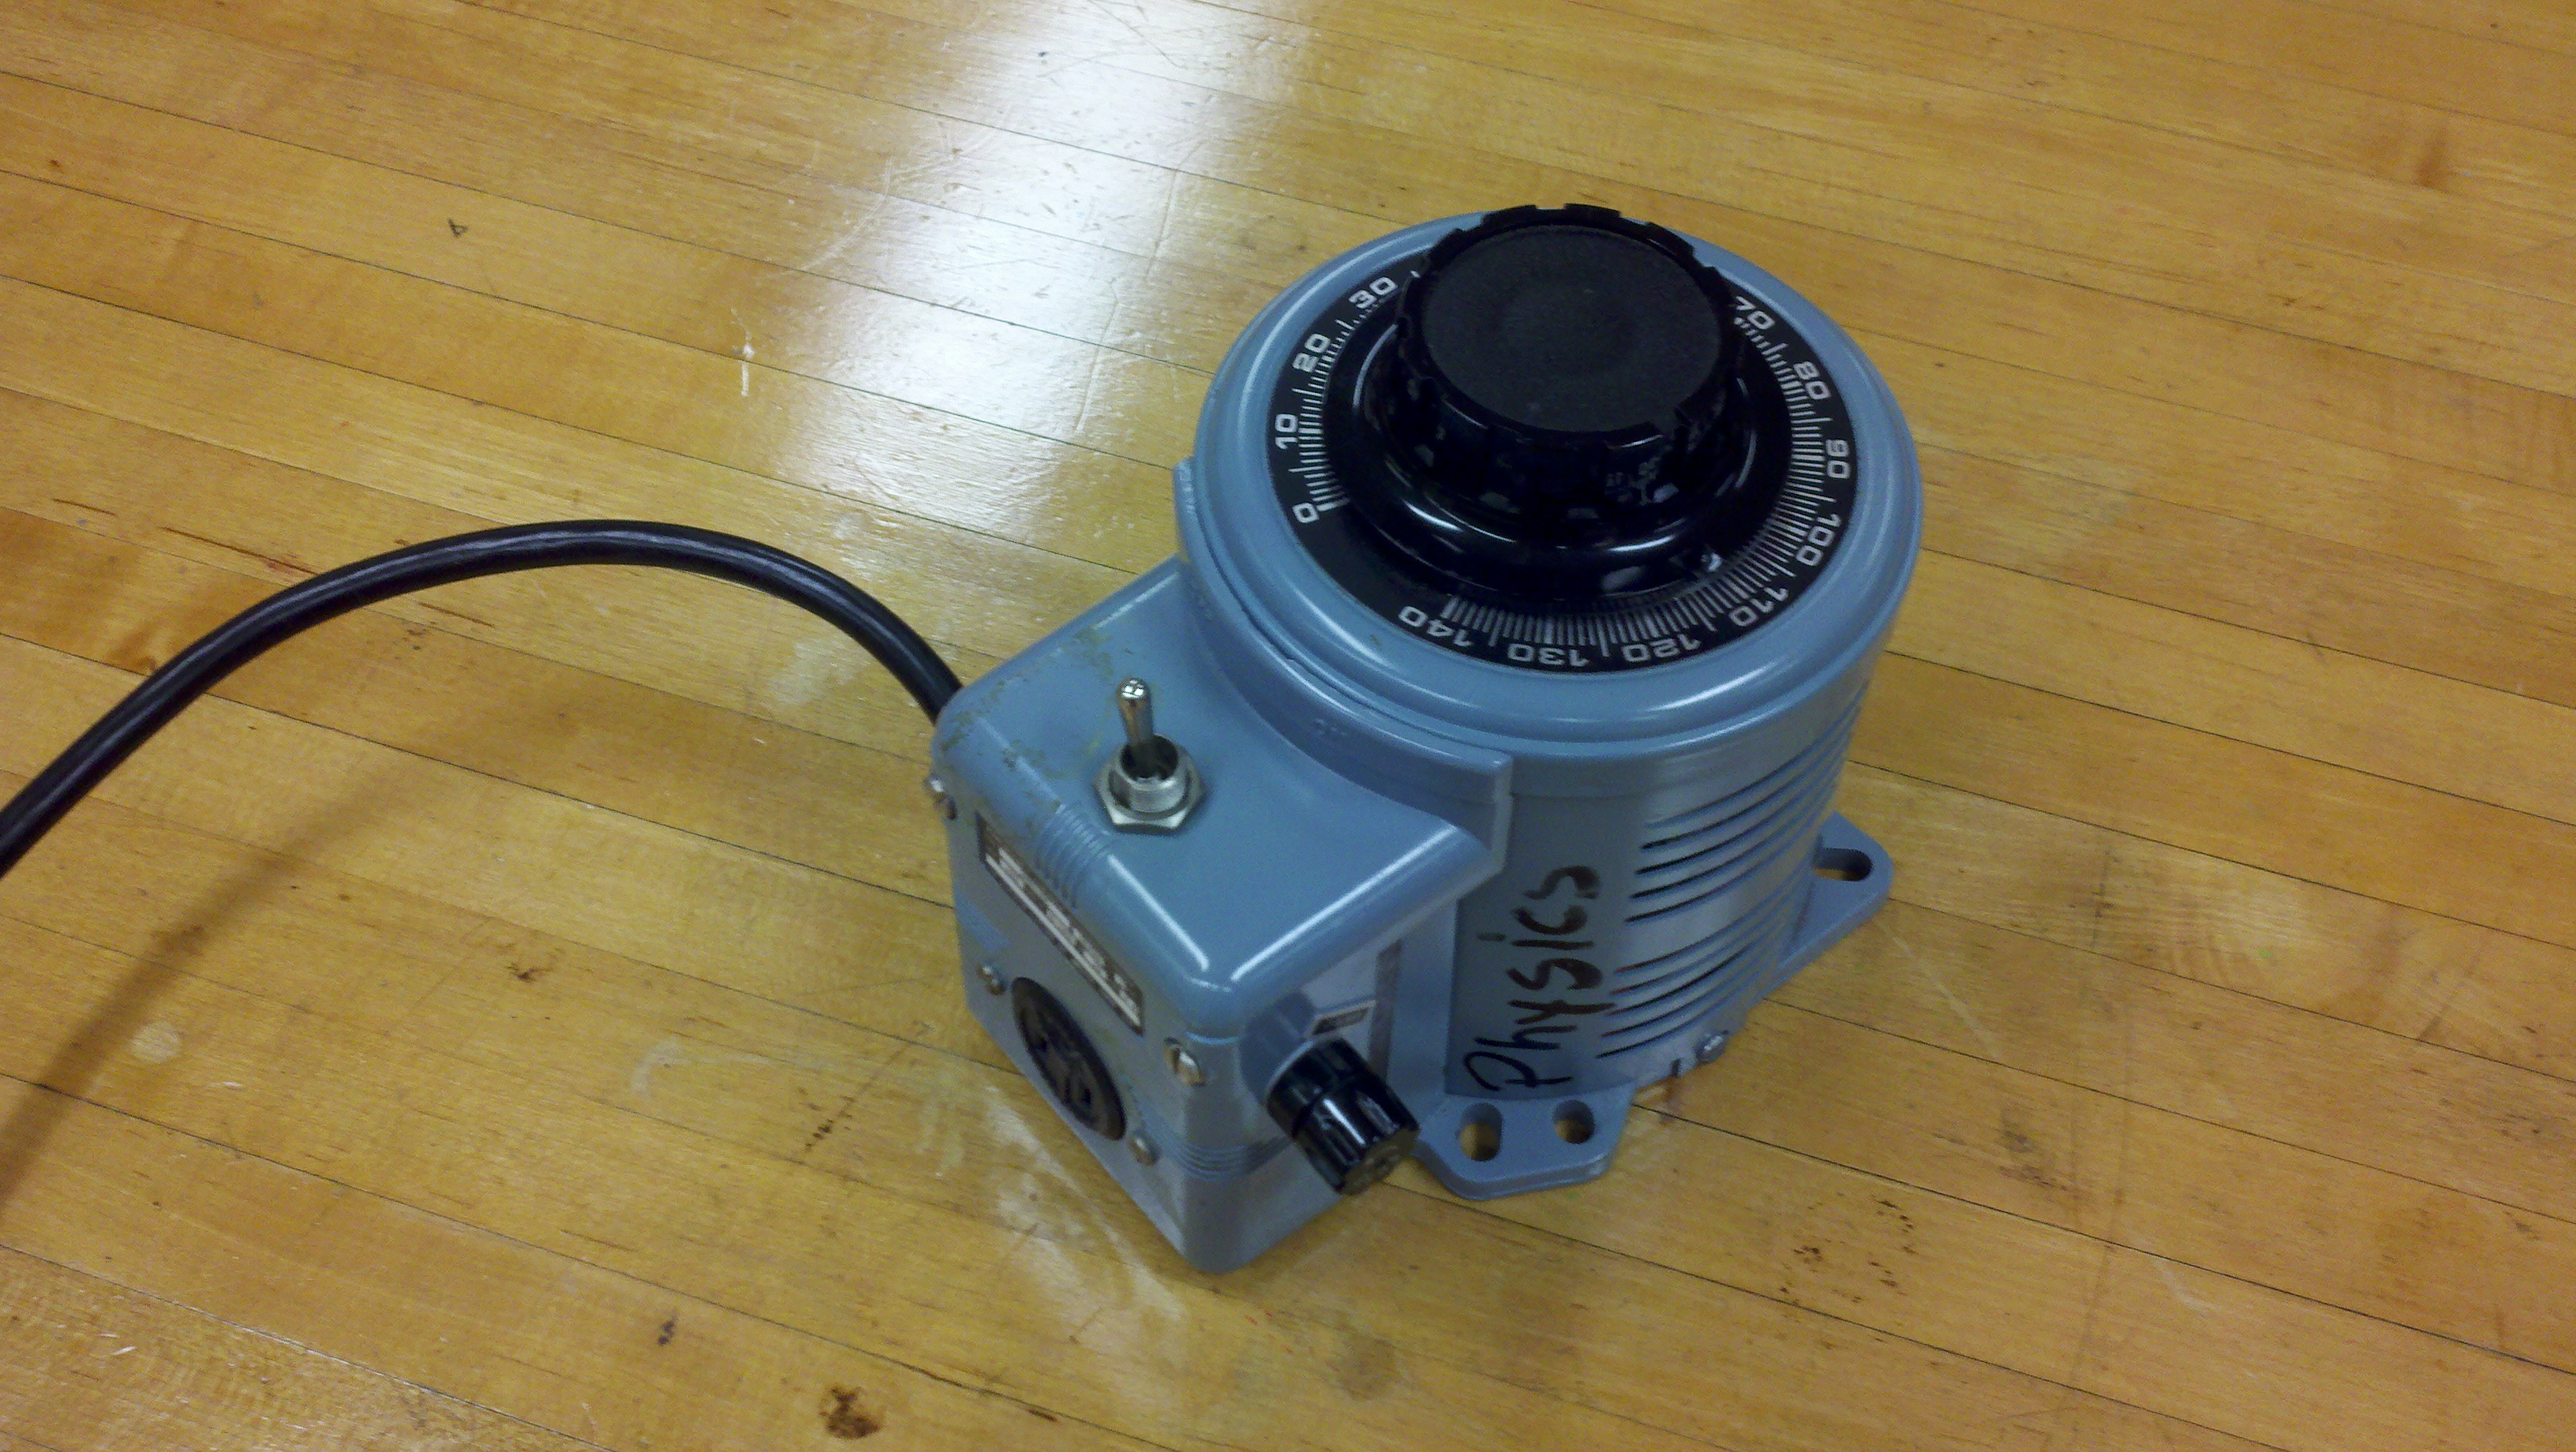
\includegraphics[width=2\textwidth/3]{figures/variac}
%% Photo by Kevin R. Lynch, 2012
  \caption{The variable transformer, aka variac.}
  \label{fig:variac}
\end{figure}
For this set of measurements, you should receive a set of incandescent
bulbs (\unit[25]{W}, \unit[40]{W}, \unit[60]{W}, \unit[75]{W}, and
\unit[100]{W}), a variac (variable transformer; see
Figure~\ref{fig:variac}), two multimeters, a lamp socket board and
connecting wires.
\begin{quote}
  Warning!  The light bulbs \textit{will} get \textbf{hot}!  Be
  careful when you unscrew them so you don't get burnt.  In addition,
  there will be unprotected \unit[120]{V} sources present.  Just as
  you wouldn't stick you fingers in a wall socket, \textbf{do not}
  touch the bare wires or terminals!  Don't stick any part of your
  hand \textit{under} the acrylic sheets!  Don't disconnect the wiring
  from the variac without turning it off!
\end{quote}

%%
\begin{table}
  \centering
  \caption{The new circuit schematic symbols for this lab.}
  \begin{tabular}{|l|c|}\hline
    Variac & 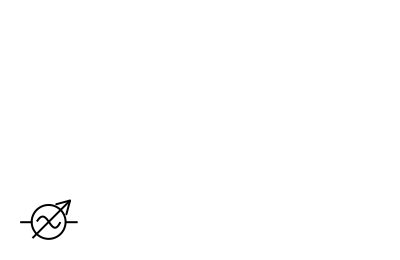
\includegraphics[width=1in]{figures/variac_schem}\\ \hline
%% Figure derived from 
%% http://en.wikipedia.org/wiki/File:Circuit_elements.svg
%% under GNU Free Documentation License
    Lamp & 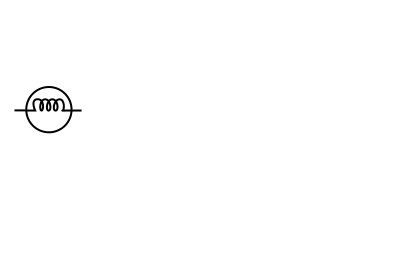
\includegraphics[width=1in]{figures/lamp}\\ \hline
  \end{tabular}
  \label{tab:symbols}
\end{table}
%%
\begin{figure}
  \centering
  \includegraphics[width=2\textwidth/3]{figures/circuit}
%% Figure derived from 
%% http://en.wikipedia.org/wiki/File:Circuit_elements.svg
%% under GNU Free Documentation License
  \caption{The circuit including the incandescent lamp powered by the variac.}
  \label{fig:circuit}
\end{figure}
%% 
\begin{table}
  \centering
  \caption{The filament data table.}
  \label{tab:filament}
  \begin{tabular}{|l|r|r|r|} \hline
    \begin{tabular}{c}Lamp\\Wattage\end{tabular} & 
    \begin{tabular}{c}
      Operating\\Temperature [\unit{\textdegree C}]
    \end{tabular} &
    \begin{tabular}{c}
      Length of\\uncoiled\\filament [\unit{m}]
    \end{tabular} & 
    Cross-section [$\unit{m^2}$] \\ \hline
    25 & 2290 & 0.56 & $7.00 \times 10^{-10}$\\ \hline
    40 & 2470 & 0.38 & $8.56 \times 10^{-10}$ \\ \hline
    60 & 2550 & 0.53 & $1.60 \times 10^{-9}$ \\ \hline
    75 & 2600 & 0.55 & $2.23 \times 10^{-9}$ \\ \hline
    100 & 2650 & 0.58 & $3.17 \times 10^{-9}$ \\ \hline
  \end{tabular}  
\end{table}

\begin{enumerate}
\item Measure and record the ambient temperature.  Why do you need
  this? 
\item Directly measure the resistance of each of your lamps.  Using
  the data in Table~\ref{tab:filament} you can determine the
  resistivity of tungsten as predicted by each lamp individually.  Are
  your measurements consistent?  If not, what might be the problem?
\item Build the circuit shown in Figure~\ref{fig:circuit}, which will
  be run at \unit[120]{V}.  The multimeter measuring voltage should be
  set to the \texttt{AC V} setting and \unit[200]{V} \texttt{Range};
  the multimeter measuring current should be set to the \texttt{AC A}
  setting, and an appropriate range determined from the voltage and
  resistance of the lamp.
  \begin{quote}
    \textbf{DO NOT plug in the variac or turn on the circuit until it
      has been checked by your instructor!}
  \end{quote}
\item Turn on the circuit, and set the voltage to \unit[120]{V}.
  Measure and record both the voltage and current values.  Repeat with
  all of the lamps.  You will be determining the temperature dependent
  resistance of the filaments, and extracting the temperature
  coefficient of resistivity.
\end{enumerate}

\subsection{Variations on a theme}
\label{sec:variations}

\begin{figure}
  \centering
  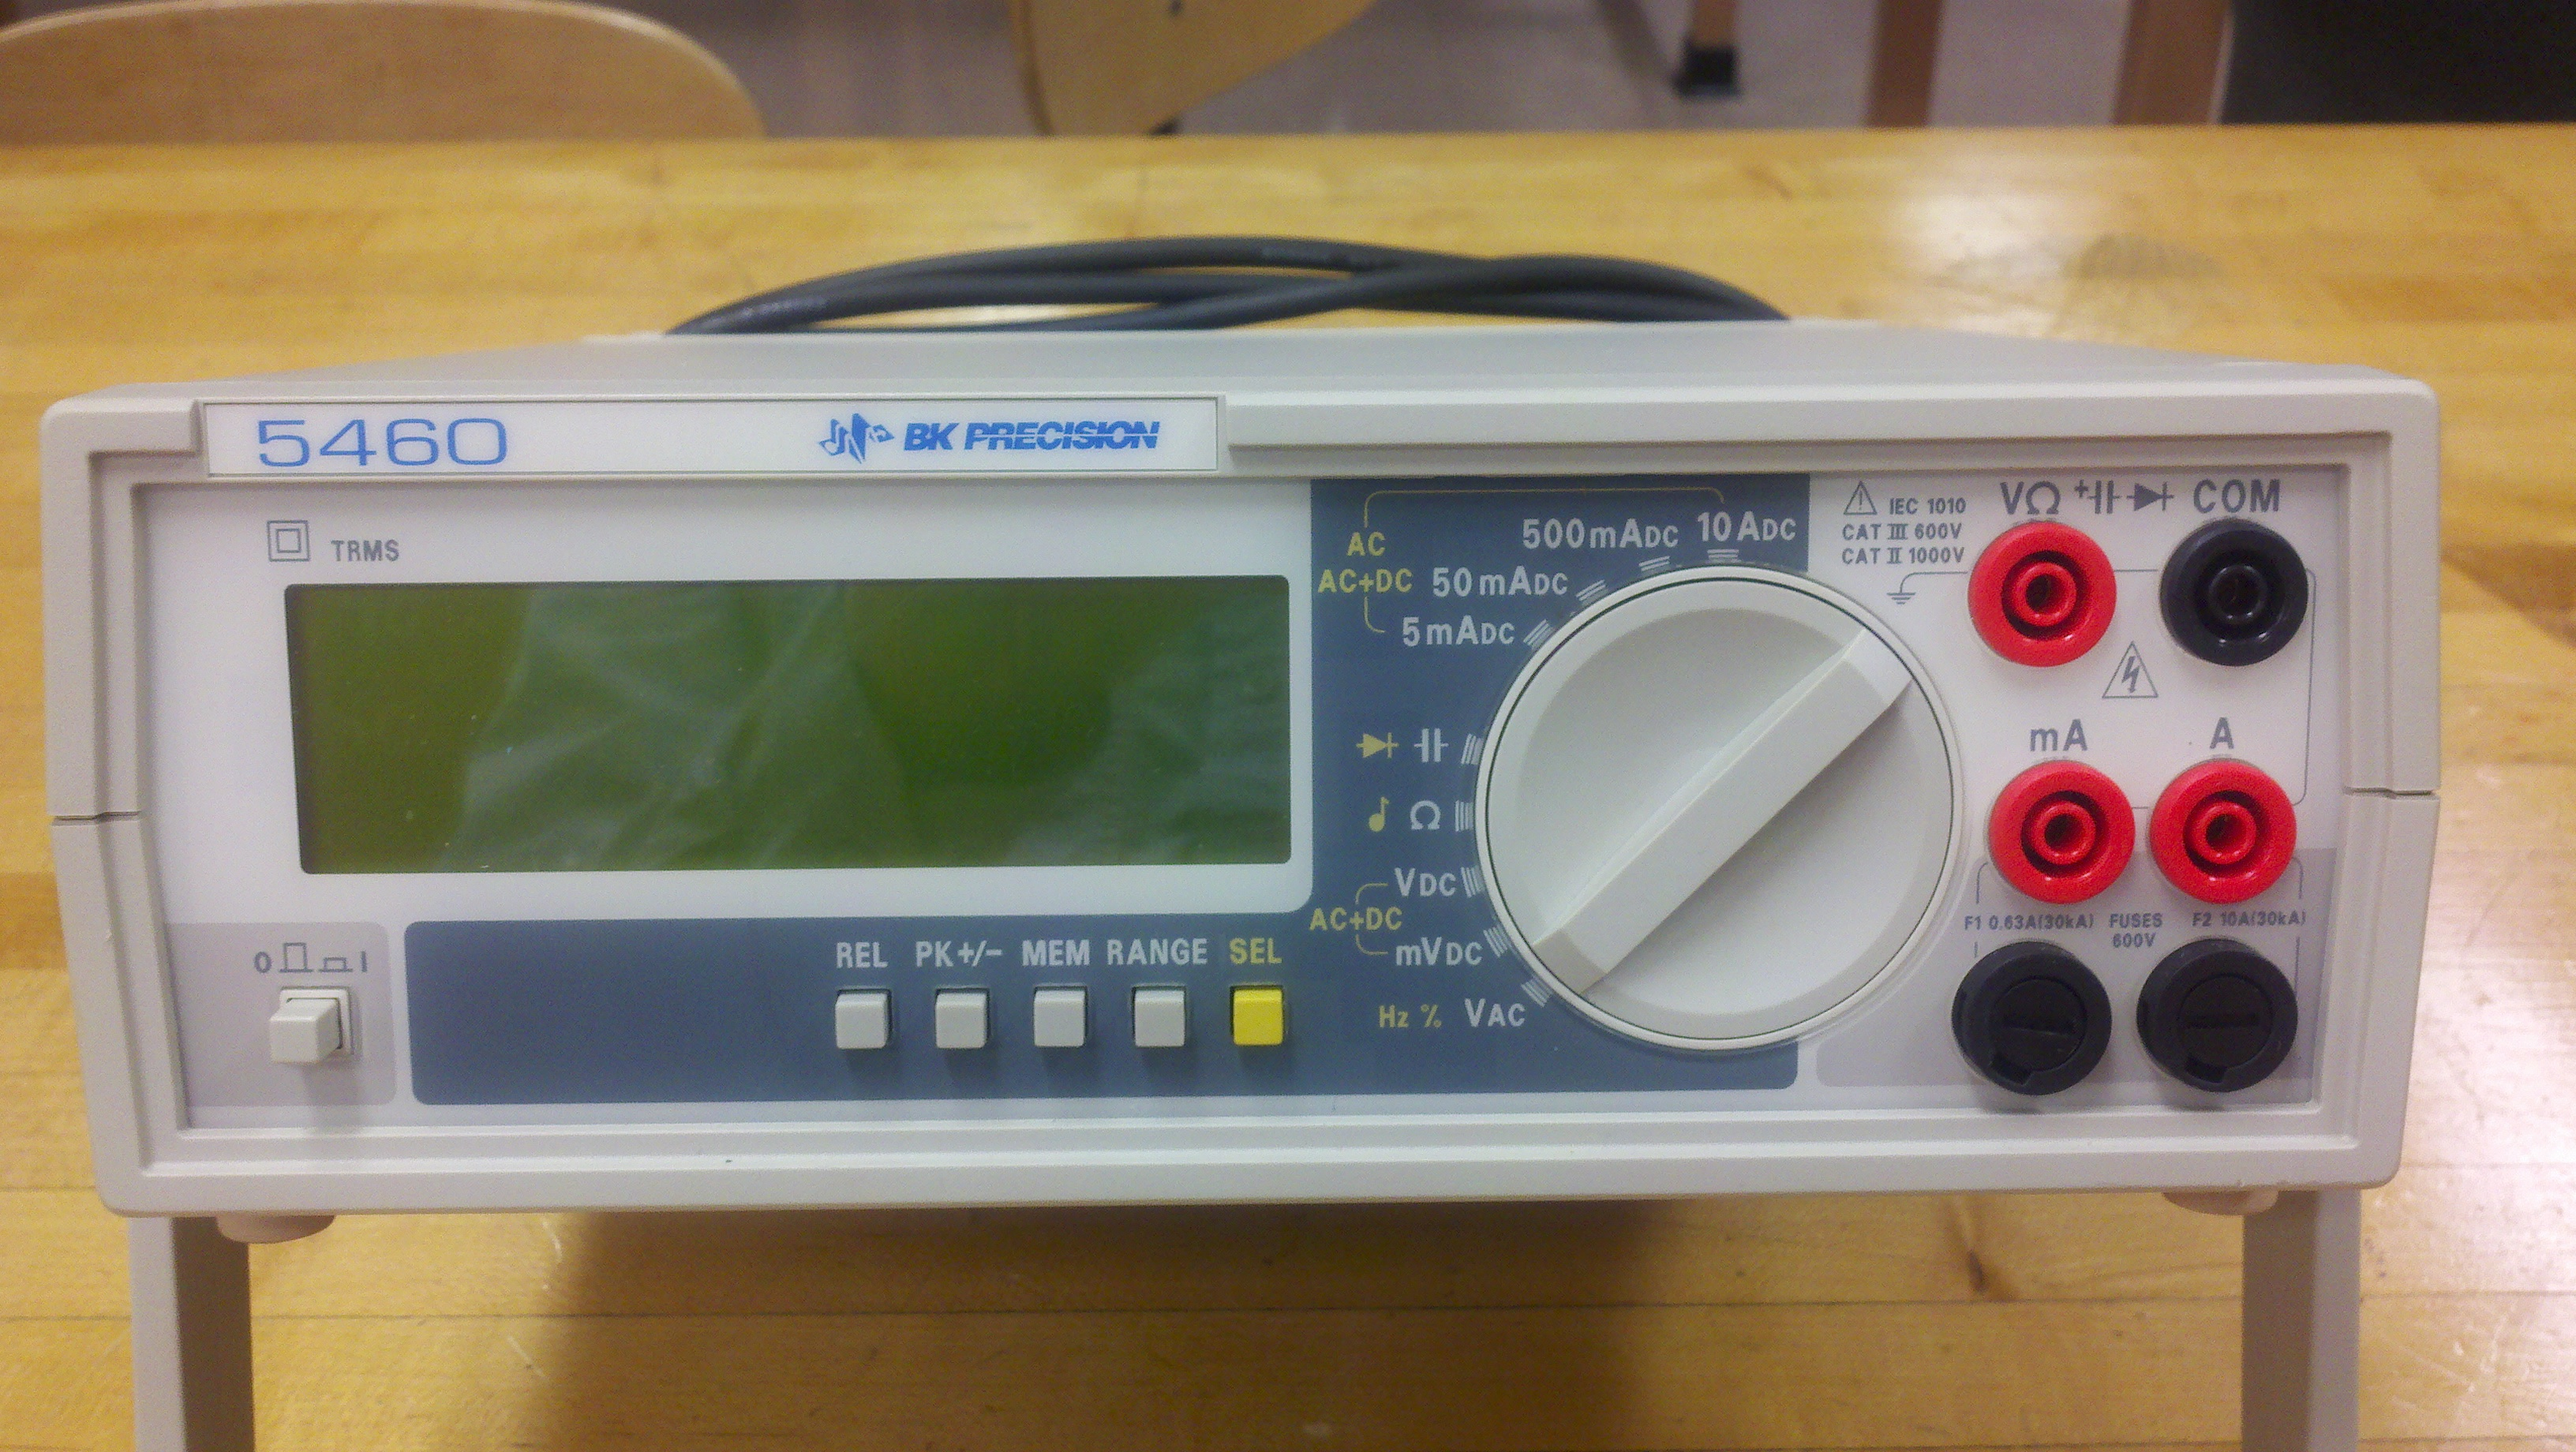
\includegraphics[width=2\textwidth/3]{figures/bk_5460}
%% Photo by Kevin R. Lynch, 2012
  \caption{The high percision BK Precision 5460 multimeter.}
  \label{fig:multimeter}
\end{figure}
In this section, you will be responsible for answering the following
question: what is the resistivity of material $X$?  You will have
available a high precision multimeter (see
Figure~\ref{fig:multimeter}) with probes, calipers, micrometers, and
various bibs and bobs around the lab (like wires, clips, tools, meter
sticks, stands, etc.)  You must design, implement, and critique an
experimental procedure to make a reasonable determination of the
resistivity of the current carrying material.  If you don't see
something you might find useful, \textit{ask}; we might just have it
available.

Your instructor will split your lab partnerships into groups, which
will design and implement the experiment.  Discuss, write on the
board/paper/tablet, draw, diagram, argue, convince, cajole, and then
measure and analyze the results.  Don't be passive: each student must
still produce their own writeup, indicating their own ideas and
contributions!  See the post-lab exercises for some topics of
discussion.

Here are some of the possible materials to analyze:
\begin{enumerate}
\item Pencil lead isn't; it's actually a mechanically compressed form
  of the carbon allotrope \textit{graphite}.  Graphite is not only
  flammable, it is also useful as a lubricant, and it conducts
  electricity.  Determine the resistivity of the graphite in a
  standard Number 2 pencil.
\item Most metals are \textit{ductile} as well as \textit{conductive};
  this is not a coincidence: the most conductive metals (lowest
  resistivity) also tend to be the most ductile.  Wires are
  \textit{drawn} from large diameter cylinders, first by rollers, and
  then by forcing the cylinder through a tapered bore-hole in a
  heavy-weight \textit{die}.  The result is a wire of uniform (usually
  circular) cross-section that is wrapped on a spool.  Using the
  provided lengths of wire (copper, steel,\footnote{An alloy of iron
    and carbon, with traces of other elements.} and
  nichrome.\footnote{A steel-like alloy of nickel, chromium, and
    iron.}
\begin{figure}
  \centering
  \subfloat[][External View]{
    \label{fig:calorimeter:external}
    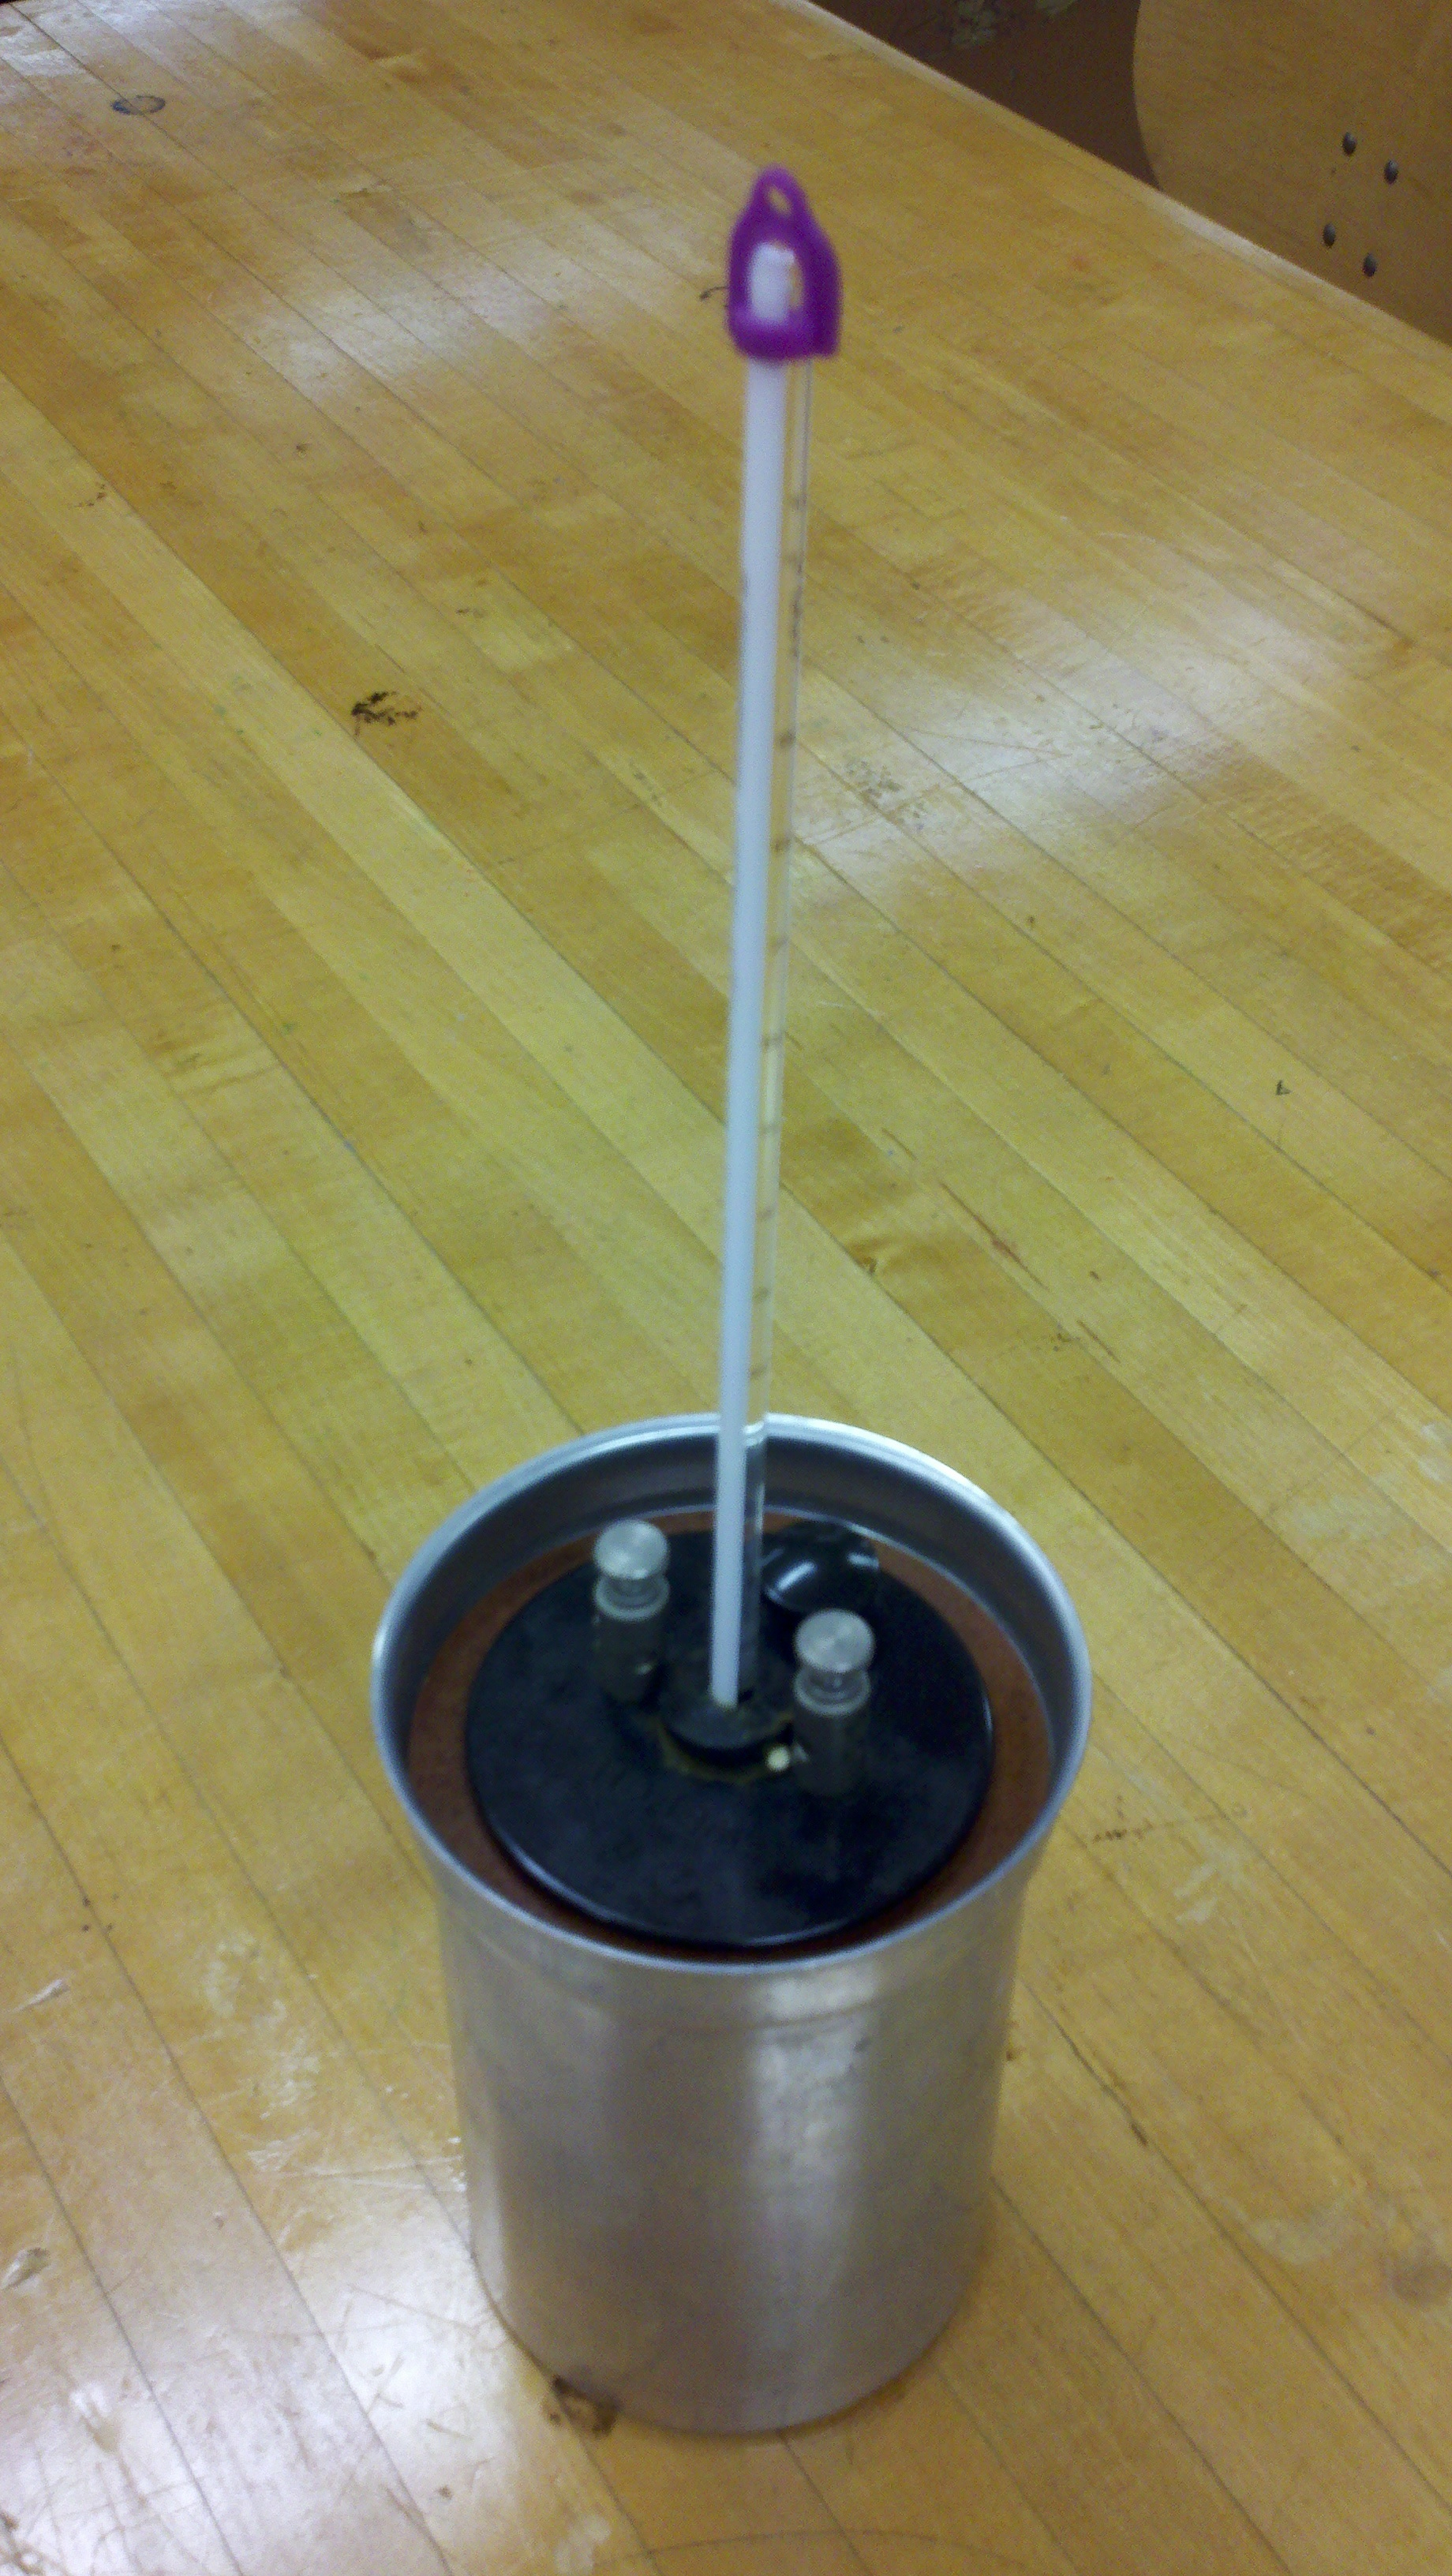
\includegraphics[width=\textwidth/3]{figures/external}
%% Photo by Kevin R. Lynch, 2012
  } \qquad
  \subfloat[][Internal View]{
    \label{fig:calorimeter:internal}
    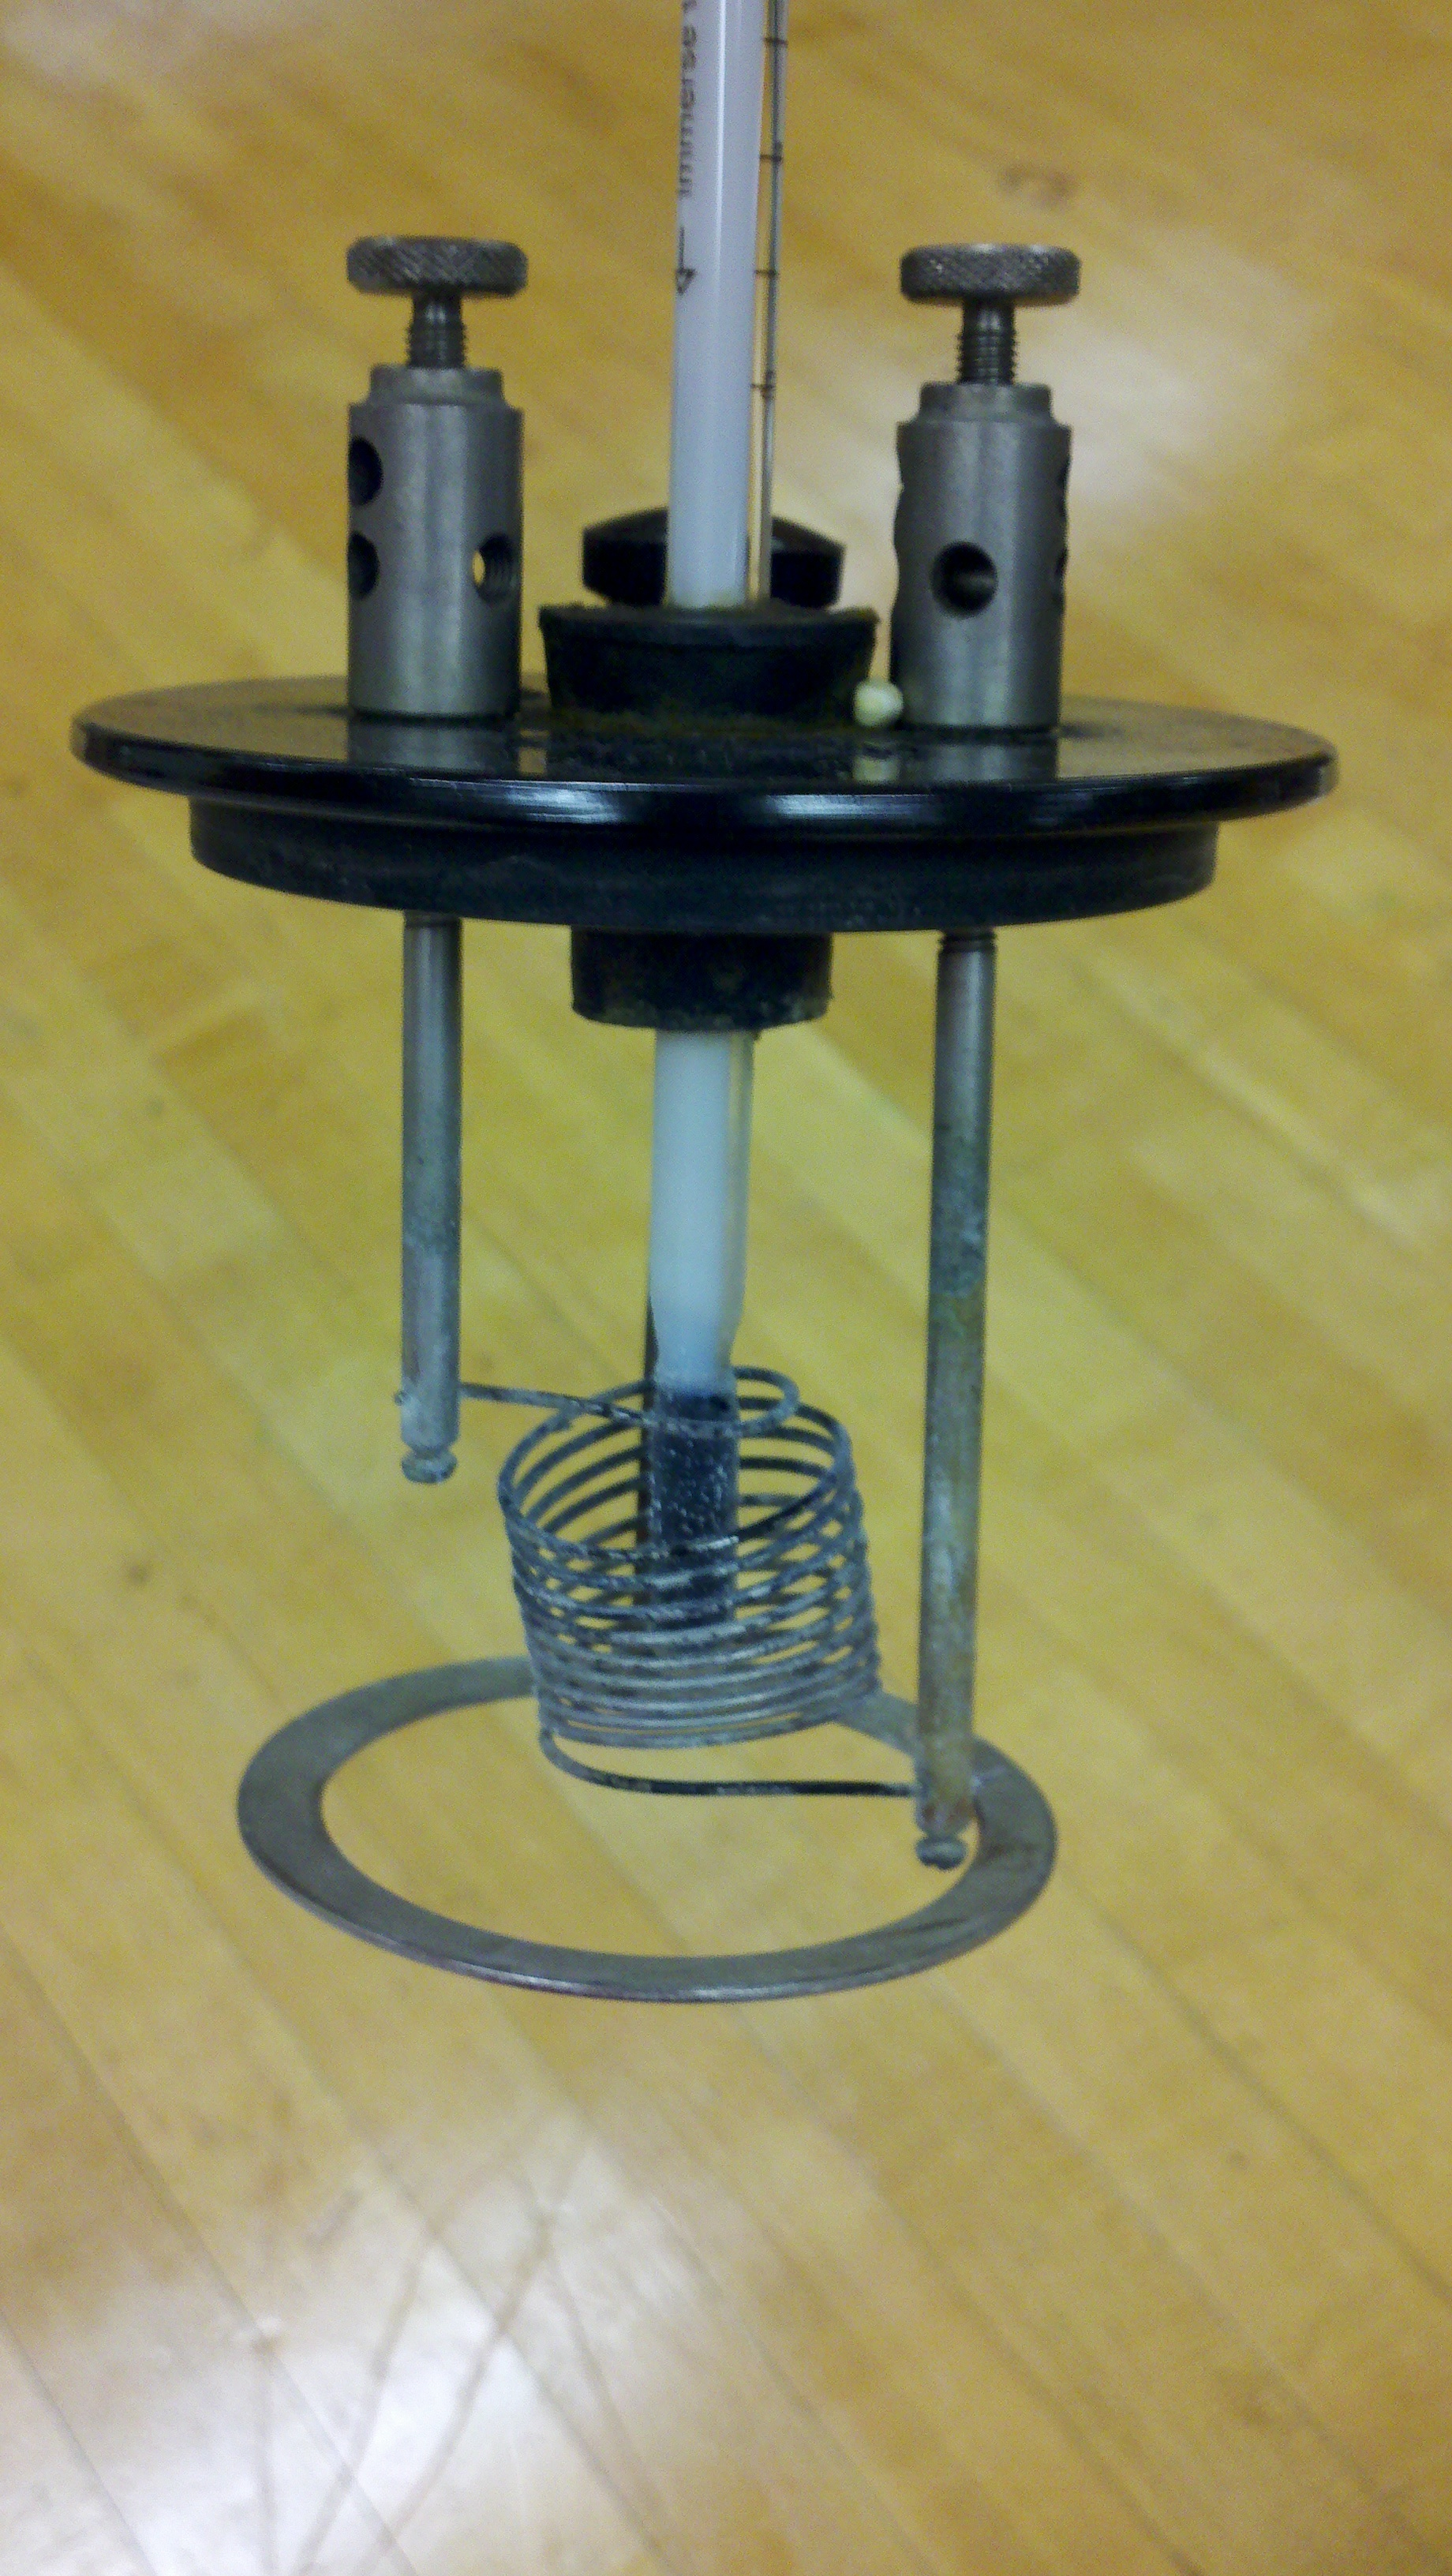
\includegraphics[width=\textwidth/3]{figures/internal}
%% Photo by Kevin R. Lynch, 2012
  }
  \caption{Internal and external views of the calorimeter.}
  \label{fig:calorimeter}
\end{figure}
\item Sometimes, getting access to the wire whose resistivity you want
  to measure requires some clever thought.  Last semester, you
  performed a calorimetry experiment, where you heated the insulated
  volume using an immersed wire coil.  Without cutting or
  disassembling the calorimeter, determine the resistivity of the
  coil material.  Note: the conductive posts that \textit{hold} the
  coil are a different material, and their effect should be eliminated
  in your measurements.
\item Sometimes, it isn't the resistivity of the material you're after:
  remember, Equation~\eqref{eq:resistivity} relates four different
  quantities; given any three, you can determine the remaining one.
  Given a spool of copper wire of known resistivity
  ($\unit[16.8]{n\Omega \cdot m}$ at \unit[20]{\textdegree C}),
  determine the length of the wire on the spool.
\end{enumerate}

\newpage

\section*{Pre-Lab Exercises}

Answer these questions as instructed on Blackboard; make sure to
submit them before your lab session!

\begin{enumerate}
\item What's the difference between \textit{intrinsic} and
  \textit{extrinsic} properties of a material?
\item We give a relation between dissipated power in, voltage across, and
  current through, a resistor.  Ohm's Law gives a relationship between
  the voltage, current, and resistance.  Express dissipated power in
  terms of the voltage and resistance; in terms of the current and
  resistance. 
\item A perfect conductor has zero resistivity, while a real conductor
  has a finite, but near zero resistivity.  What resistivity should a
  perfect insulator have?  Should a real insulator have a very large
  or very small resistivity?
\end{enumerate}

\newpage

\section*{Post-Lab Exercises}

\begin{enumerate}
\item Use the data you collected to determine the resistivity of
  tungsten; be sure to include an estimate of the measurement
  uncertainty, and discuss how you determined that uncertainty.
\item Use the data you collected to determine the temperature
  coefficient of resistivity for tungsten; be sure to include an
  estimate of the uncertainty, and discuss how you determined that
  uncertainty.  Since you have the resistivity at six temperatures,
  you should produce at least one (and better, two!) plots of the
  resistivity versus temperature; is it linear?  Are you sure?  Can
  you extrapolate from the high operating temperatures down to room
  temperature? 
\item By measuring the voltage and current used for each lamp, you can
  calculate the actual dissipated power.  How does this compare to the
  advertised value?  Stefan's Law (look back at your Physics I text)
  relates the electromagnetic power dissipation to the surface
  temperature of an object; since you have both, you can calculate the
  emissivity of each lamp filament.  Are they the same?  Speculate on
  the source of any differences.
\item For the experiment you designed, write a brief ``Lab Manual'':
  state the objectives, write a brief overview of the theory, describe
  your hypothesis testing procedure.  State your results, including
  any estimate of the uncertainty, and how you reached those
  estimates.  
\item Discuss briefly whether you have met the objectives of the lab
  exercises. 
\end{enumerate}

\end{document}

%%% Local Variables: 
%%% mode: latex
%%% TeX-master: t
%%% End: 
